\section{Сбор и подготовка данных}

Для решения помлавленой задачи первоночально был проведен опрос Операторов БПЛА из ПСО "Лиза Алерт", а также получены несколько примеров снимков. В результате были выяснены следующие аспекты:

\begin{itemize}
    \item Условия сьемки;
    \begin{itemize}
        \item Высота -- 40-50 метров над поверхностью земли;
        \item Съекмка производиться вертикально (вид сверху);
        \item Во время съемки БПЛА зависает над сценой и сфокусироваться;
    \end{itemize}
    \item Позы, в которых чаще всего находят потерявшихся людей;
    \begin{itemize}
        \item Стоящий человек (идущий, бегущий);
        \item Сидячий человек (на корточках);
        \item Лежачий человек (на спине);
        \item Лежачий человек (на животе);
        \item Лежачий человек (на боку);
        \item Лежачий в позе эмбриона человек.
    \end{itemize}
\end{itemize}

При поиске доступных открытых решений удалось найти 2 набора данных (dataset-а): SDD (stenford Drone Dataset) и VisDrone DET dataset, но ни один из них не подходил для решения пославленой задачи (рис. \ref{sdd-visdrone-example}). В этих наборах данных несколько отличались условия съемки а также отсутствовали отсутсвовала как природная среда так и интересующие нас позы. Однако у них одно существенное приемущество -- по схожести задачи они были значительно ближе, чем какие-либо другие. По этому в описанных ниже исследованиях они использовались для предобучения моделей (а как следствие и сужения доменной области) и оценки качества моделей. Также открытость этих данных и их известность позволила сравнивать качество полученных моделей с уже имеющимися.

\begin{figure}[H]
    \centering
    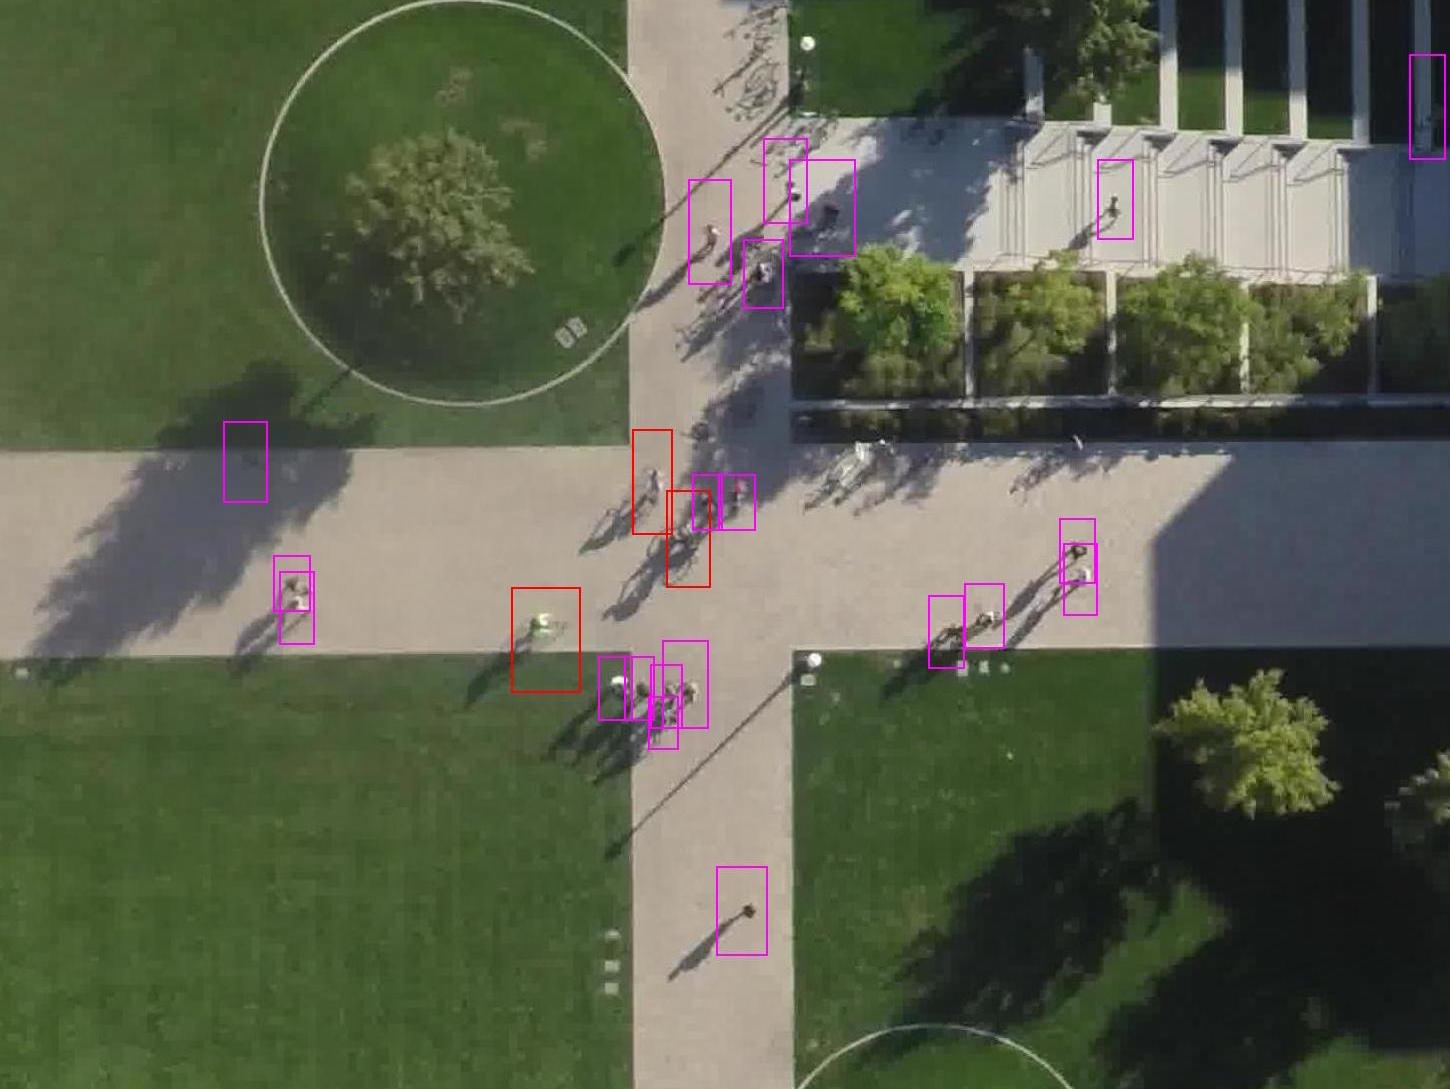
\includegraphics[width=0.42\linewidth]{3-sdd-example}
    \hfill
    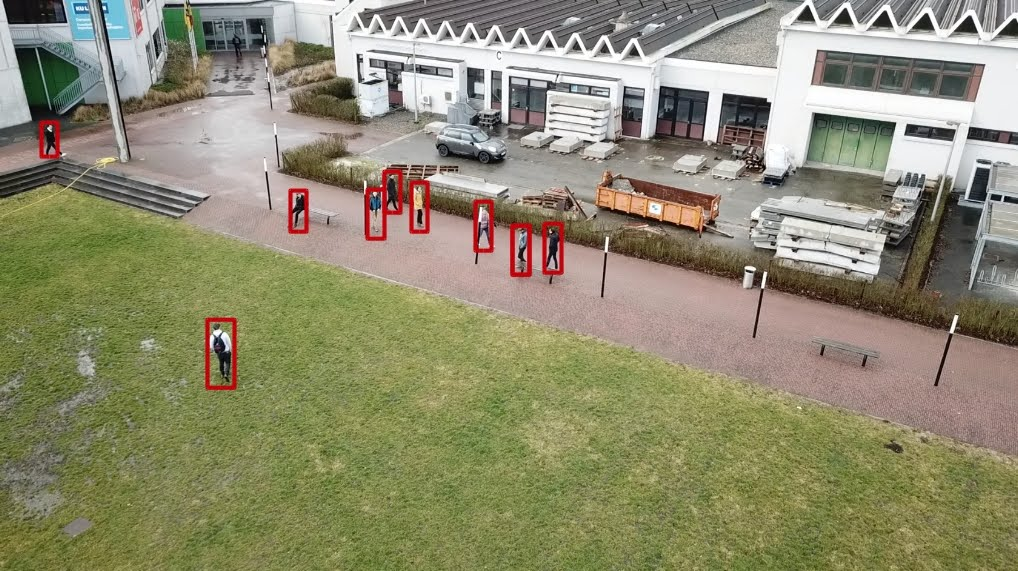
\includegraphics[width=0.56\linewidth]{3-visdrone-example}
    \caption{Примеры изображений SDD и VisDrone наборовтданных} \label{sdd-visdrone-example}
\end{figure}


В силу специфичности решаемой задачи пришлось самостоятельно формировать и организовывать сбор датасета с необходимыми нам фотографиями. Для решения этой задачи были привлечены добровольцы из различных ПСО, а также разработаны методические материалы по сбору и разметке данных.

В результате был получен уникальный в своем роде набор данных получивший в последствии название Lacmus Drone Dataset (LaDD). LaDD состоит из 1431 фотографии и меет формат аннотирования Pascal VOC с одним классом "Pedestrian" (пешиход). Dataset также яаляется открытым и распросраняется по лицензии GNU GPL v3. В его создании приняло участие множество ПСО из различных регионов России (Москва, Саратов, Ямал, Крым, Калининград и др). Таким образом удолось достичь высокого разнообразия природных условий и как следствие и обучающей выборки. Ниже приведен пример фотографий:

\addimghere{3-ladd-example}{1}{Московская область, осень 2019, бурелом, лежачий на боку человек}{ladd-example}